\chapter{Fluidos perfectos: Euler y Bernoulli}\label{ch:b2:euler-bernoulli}

Sujétese una hoja de papel por un borde y sóplese por encima: se levanta.
Ábrase el grifo de la ducha y la cortina se mete hacia dentro. Un ala
sostiene trescientas toneladas porque el aire circula más deprisa por su
extradós que por su intradós. Los tres casos dicen lo mismo: \emph{donde
un fluido se mueve más deprisa, su presión es menor}. Este capítulo
escribe la segunda ley de Newton para una \omterm{def:b2:fluid-kinematics:particle}{partícula de fluido} en el modelo
más sencillo --- el fluido \emph{perfecto}, que siente la presión pero no
el rozamiento --- y extrae de ella el \omterm{thm:b2:euler-bernoulli:bernoulli}{teorema de Bernoulli}, el balance
energético de una \omterm{def:b2:fluid-kinematics:euler}{línea de corriente}, cuyas aplicaciones van del
caudalímetro de una tubería al indicador de velocidad de un avión.

\section{La ecuación de Euler}

\begin{proposition}[Fuerza de presión sobre una partícula de fluido]\label{prop:b2:euler-bernoulli:pressure}
\index{fuerza de presión (densidad volumétrica)}
La resultante de las fuerzas de presión que el fluido circundante ejerce
sobre una partícula de volumen $\dd\tau$ vale
\[
\dd\vect F_P = -\operatorname{\vect{grad}}P\,\dd\tau :
\]
la presión actúa como una fuerza volumétrica de densidad $-\operatorname{\vect{grad}}P$,
que empuja desde las presiones altas hacia las bajas.
\end{proposition}

\begin{proof}
Sobre la caja de \cref{thm:b2:fluid-kinematics:continuity}, las caras
situadas en $x$ y en $x + \dd x$ reciben $+P(x)\dd y\dd z$ y $-P(x + \dd x)\dd y\dd z$
según $x$: en total $-\partial_xP\,\dd x\dd y\dd z$; e igual para $y$ y $z$.
\end{proof}

\begin{definition}[Fluido perfecto]\label{def:b2:euler-bernoulli:perfect}
\index{fluido perfecto}
Un \emph{fluido perfecto} es aquel en el que la única fuerza de contacto
entre partículas vecinas es la presión --- normal a toda superficie, sin
esfuerzo tangencial (viscoso). Es una idealización válida, como explica el
capítulo siguiente, lejos de las paredes y a número de Reynolds elevado:
el agua de una tubería lejos de la pared, el aire en torno a un ala fuera
de la delgada capa límite, una ola en el mar.
\end{definition}

\begin{theorem}[Ecuación de Euler]\label{thm:b2:euler-bernoulli:euler}
\index{ecuación de Euler}
En un sistema galileano, un \omterm{def:b2:euler-bernoulli:perfect}{fluido perfecto} de densidad $\rho$ sometido a
la gravedad obedece, en todo punto,
\[
\rho\Bigl(\frac{\partial\vect v}{\partial t} + (\vect v\cdot\operatorname{\vect{grad}})
\vect v\Bigr) = -\operatorname{\vect{grad}}P + \rho\vect g ,
\]
al que se añade en el segundo miembro cualquier otra densidad de fuerza
volumétrica $\vect f_v$ (eléctrica, o de inercia en un sistema no
galileano). En reposo se reduce a la ley hidrostática
$\operatorname{\vect{grad}}P = \rho\vect g$ del volumen del Año 1.
\end{theorem}

\begin{proof}
Segunda ley de Newton para la partícula de masa $\rho\,\dd\tau$: su
aceleración es la \omterm{thm:b2:fluid-kinematics:material}{derivada material}
(\cref{thm:b2:fluid-kinematics:material}) y las fuerzas son la resultante
de presión y el peso $\rho\vect g\,\dd\tau$; divídase por $\dd\tau$.
\end{proof}

\begin{example}[Un depósito que acelera]\label{ex:b2:euler-bernoulli:tank}
El agua de un depósito transportado por un camión que acelera con $\vect a$
está en reposo en el sistema del camión; allí, Euler con la fuerza de
inercia $-\rho\vect a$ da $\operatorname{\vect{grad}}P = \rho(\vect g - \vect a)$:
la presión crece en la dirección de la ``gravedad efectiva''
$\vect g - \vect a$, la superficie libre (una isobara) es perpendicular a
ella y se inclina hacia atrás el ángulo $\arctan(a/g)$ ---
\qty{11}{\degree} para $a = \qty{2}{m/s^2}$. En un cubo que gira a
$\Omega$, la fuerza centrífuga $\rho\Omega^2r\,\vect e_r$ da
$P = P_0 + \tfrac12\rho\Omega^2r^2 - \rho gz$ y la superficie libre es el
paraboloide $z = \Omega^2r^2/2g$.
\end{example}

\begin{omfigure}
\begin{tikzpicture}[font=\small, x=1cm, y=1cm, >=Stealth]
  \begin{scope}
    \draw[thick, fill=omDef!10] (0,0) rectangle (1.8,1.4);
    \draw[omThm, very thick, ->] (-1.0,0.7) -- (-0.05,0.7) node[pos=0.2, above, font=\footnotesize] {$P(x)\,\dd S$};
    \draw[omThm, very thick, ->] (2.85,0.7) -- (1.85,0.7) node[pos=0.1, above, font=\footnotesize] {$P(x+\dd x)\,\dd S$};
    \draw[omThm, very thick, ->] (0.9,-1.0) -- (0.9,-0.05);
    \draw[omThm, very thick, ->] (0.9,2.4) -- (0.9,1.45);
    \node[font=\footnotesize] at (0.9,-1.4) {$\dd\vect F_P = -\operatorname{\vect{grad}}P\,\dd\tau$};
  \end{scope}
  \begin{scope}[xshift=6.0cm]
    \draw[thick] (-1.6,-0.2) -- (-1.6,1.6) (-1.6,-0.2) -- (1.6,-0.2) -- (1.6,1.6);
    \draw[omDef, thick, fill=omDef!15] (-1.6,1.4) -- (1.6,0.2) -- (1.6,-0.2) -- (-1.6,-0.2) -- cycle;
    \draw[->, very thick] (0,1.9) -- (0.45,1.9) node[right, font=\footnotesize] {$\vect a$};
    \draw[omThm, ->, thick] (0,0.5) -- (0,-0.7) node[right, font=\footnotesize] {$\vect g$};
    \draw[omProp, ->, thick] (0,0.5) -- (-0.45,-0.7) node[left, font=\footnotesize] {$\vect g - \vect a$};
    \node[font=\footnotesize] at (0,-1.4) {depósito acelerado: superficie $\perp \vect g - \vect a$};
  \end{scope}
  \begin{scope}[xshift=11.2cm]
    \draw[thick] (-1.4,-0.2) -- (-1.4,1.8) (-1.4,-0.2) -- (1.4,-0.2) -- (1.4,1.8);
    \draw[omDef, thick, fill=omDef!15, domain=-1.4:1.4, samples=40] plot (\x,{0.35+0.6*\x*\x}) -- (1.4,-0.2) -- (-1.4,-0.2) -- cycle;
    \draw[dashed] (0,-0.5) -- (0,2.1);
    \draw[->] (-0.3,2.0) arc[start angle=150, end angle=30, radius=0.35] node[right, font=\footnotesize] {$\Omega$};
    \node[font=\footnotesize] at (0,-1.4) {cubo en rotación: $z = \Omega^2r^2/2g$};
  \end{scope}
\end{tikzpicture}

{\small A la izquierda, las fuerzas de presión sobre las caras de una caja
de fluido no se cancelan cuando $P$ varía: su resultante vale
$-\operatorname{\vect{grad}}P$ por unidad de volumen. En el centro y a la
derecha, dos fluidos en reposo en un sistema acelerado; la superficie
libre es en todo punto perpendicular a la gravedad efectiva.}
\end{omfigure}

\section{El teorema de Bernoulli}

\begin{theorem}[Bernoulli]\label{thm:b2:euler-bernoulli:bernoulli}
\index{teorema de Bernoulli}\index{presión de estancamiento}\index{presión dinámica}
Para un fluido \emph{perfecto} e \emph{incompresible}, de densidad
uniforme y en régimen \emph{estacionario}, en un sistema galileano con gravedad uniforme, la magnitud
\[
P + \tfrac12\rho v^2 + \rho gz
\]
es constante \emph{a lo largo de cada \omterm{def:b2:fluid-kinematics:euler}{línea de corriente}}. Si además el
flujo es \emph{irrotacional}, la constante es la misma en todo el fluido.
El término $\tfrac12\rho v^2$ es la \emph{\omterm{thm:b2:euler-bernoulli:bernoulli}{presión dinámica}}; $P + \tfrac12\rho v^2$
es la \emph{\omterm{thm:b2:euler-bernoulli:bernoulli}{presión de estancamiento}}, la presión que alcanzaría el fluido
si se lo detuviera a lo largo de su \omterm{def:b2:fluid-kinematics:euler}{línea de corriente}.
\end{theorem}

\begin{proof}
Euler estacionario con $(\vect v\cdot\operatorname{\vect{grad}})\vect v =
\operatorname{\vect{grad}}(v^2/2) + \vect\omega\wedge\vect v$ y $\rho\vect g =
-\operatorname{\vect{grad}}(\rho gz)$, con $\rho$ uniforme:
\[
\operatorname{\vect{grad}}\bigl(P + \tfrac12\rho v^2 + \rho gz\bigr) = -\rho\,
\vect\omega\wedge\vect v .
\]
El segundo miembro es perpendicular a $\vect v$, de modo que el gradiente
de la magnitud de Bernoulli no tiene componente a lo largo de la \omterm{def:b2:fluid-kinematics:euler}{línea de
corriente}: la magnitud es constante sobre ella. Si $\vect\omega = \vect 0$
el gradiente se anula en todas partes.
\end{proof}

\begin{remark}[Lo que dice y lo que no dice Bernoulli]\label{rem:b2:euler-bernoulli:meaning}
Dividido por $\rho$, el teorema dice: la energía mecánica por unidad de
masa, $v^2/2 + gz$, más $P/\rho$ se conserva a lo largo del camino de una
partícula. El término de presión es el trabajo que realiza \emph{sobre} la
partícula la presión del fluido que la sigue, menos el que ella realiza
sobre el fluido que la precede: el teorema de la energía para una
partícula empujada a través de un campo de presión sin rozamiento. Cuatro
condiciones: \omterm{def:b2:euler-bernoulli:perfect}{fluido perfecto} (sin pérdida viscosa), estacionario,
incompresible y \emph{a lo largo de una \omterm{def:b2:fluid-kinematics:euler}{línea de corriente}}. Comparar dos
puntos de \omterm{def:b2:fluid-kinematics:euler}{líneas de corriente} distintas solo está permitido en \omterm{def:b2:fluid-kinematics:vorticity}{flujo
irrotacional}. No dice que ``el aire rápido succione'': dice que una
partícula que ha sido \emph{acelerada} (por una caída de presión) está
ahora a menor presión --- la causa es el campo de presión, la celeridad es el efecto.
\end{remark}

\begin{remark}[Fluidos compresibles]\label{rem:b2:euler-bernoulli:compressible}
Para un gas la densidad varía, pero si el flujo es estacionario, perfecto
e isentrópico la misma demostración da la conservación de $h + v^2/2 + gz$
a lo largo de una \omterm{def:b2:fluid-kinematics:euler}{línea de corriente}, siendo $h$ la entalpía por unidad de
masa ($h = c_PT$ para un gas perfecto): la forma que se usará para toberas
y turbinas en \cref{ch:b2:open-systems}. A celeridades muy inferiores a la
del sonido ($v \lesssim \qty{100}{m/s}$ en el aire) la densidad cambia
menos de un $5\%$ y el teorema incompresible es preciso.
\end{remark}

\section{Aplicaciones}

\begin{proposition}[El tubo de Venturi]\label{prop:b2:euler-bernoulli:venturi}
\index{efecto Venturi}\index{tubo de Venturi}
En una tubería horizontal que se estrecha de la sección $S_1$ a $S_2 < S_1$,
la celeridad aumenta ($v_2 = v_1S_1/S_2$, conservación de la masa) y la
presión baja:
\[
P_1 - P_2 = \tfrac12\rho(v_2^2 - v_1^2) = \tfrac12\rho v_1^2\Bigl(\frac{S_1^2}{S_2^2} - 1\Bigr) ,
\qquad
D_V = S_1v_1 = S_1S_2\sqrt{\frac{2(P_1 - P_2)}{\rho(S_1^2 - S_2^2)}} .
\]
Medir la diferencia de presión con un manómetro da el caudal: es un
\emph{\omterm{prop:b2:euler-bernoulli:venturi}{tubo de Venturi}}. El mismo efecto hace funcionar un carburador, un
pulverizador de pintura, la entrada de aire de un mechero Bunsen y la
``succión'' de un tren que pasa.
\end{proposition}

\begin{proof}
Bernoulli a lo largo de una \omterm{def:b2:fluid-kinematics:euler}{línea de corriente} central a altura constante, con $v_2 =
v_1S_1/S_2$; despéjese $v_1$.
\end{proof}

\begin{proposition}[El tubo de Pitot]\label{prop:b2:euler-bernoulli:pitot}
\index{tubo de Pitot}
Un tubo enfrentado a la corriente y cerrado por el extremo opuesto detiene
el fluido en su boca (un \emph{punto de estancamiento}); una segunda
abertura lateral, paralela a la corriente, mide la presión estática $P$.
La diferencia es la \omterm{thm:b2:euler-bernoulli:bernoulli}{presión dinámica}:
\[
P_{\text{est}} - P = \tfrac12\rho v^2 , \qquad v = \sqrt{2(P_{\text{est}} - P)/\rho} .
\]
Todo avión mide así su velocidad respecto del aire.
\end{proposition}

\begin{proof}
Bernoulli a lo largo de la \omterm{def:b2:fluid-kinematics:euler}{línea de corriente} que termina en el punto de
estancamiento, donde $v = 0$; los orificios laterales no perturban la
corriente, que pasa con los valores $v$ y $P$ sin perturbar.
\end{proof}

\begin{proposition}[Fórmula de Torricelli]\label{prop:b2:euler-bernoulli:torricelli}
\index{fórmula de Torricelli}\index{vaciado por un orificio}
Un gran depósito abierto se vacía por un orificio pequeño situado a la
profundidad $h$ bajo la superficie libre; el chorro sale con celeridad
\[
v = \sqrt{2gh} ,
\]
la celeridad de caída libre desde la superficie. El caudal vale $D_V \approx
\alpha s\sqrt{2gh}$, con $s$ el área del orificio y $\alpha \approx 0.6$ el
\emph{coeficiente de contracción} de un orificio de borde vivo (las \omterm{def:b2:fluid-kinematics:euler}{líneas
de corriente} siguen convergiendo tras el orificio).
\end{proposition}

\begin{proof}
Bernoulli desde la superficie libre (en reposo, pues el depósito es
grande: $v_{\text{sup}} = v\,s/S \ll v$; presión $P_0$) hasta el chorro (presión $P_0$
justo a la salida del orificio): $P_0 + \rho gh = P_0 + \tfrac12\rho v^2$. El flujo
es cuasiestacionario: $h$ varía despacio.
\end{proof}

\begin{omfigure}
\begin{tikzpicture}[font=\small, x=1cm, y=1cm, >=Stealth]
  \begin{scope}
    % Venturi
    \draw[thick] (-2.6,0.7) -- (-1.2,0.7) -- (-0.3,0.3) -- (0.5,0.3) -- (1.4,0.7) -- (2.6,0.7);
    \draw[thick] (-2.6,-0.7) -- (-1.2,-0.7) -- (-0.3,-0.3) -- (0.5,-0.3) -- (1.4,-0.7) -- (2.6,-0.7);
    \draw[omThm, thick, ->] (-2.3,0) -- (-1.5,0) node[above, font=\footnotesize] {$v_1$};
    \draw[omThm, thick, ->] (-0.5,0) -- (0.9,0) node[above, font=\footnotesize, yshift=-1pt] {$v_2$};
    % manometer
    \draw[thick] (-1.8,0.7) -- (-1.8,1.2) -- (-1.8,2.2); \draw[thick] (0.1,0.3) -- (0.1,2.2);
    \draw[thick] (-1.8,1.2) -- (-1.8,1.25); 
    \fill[omDef!40] (-1.85,0.7) rectangle (-1.75,1.9); \fill[omDef!40] (0.05,0.3) rectangle (0.15,1.2);
    \draw[<->] (0.5,1.2) -- (0.5,1.9) node[midway, right, font=\footnotesize] {$\Delta h$};
    \draw[dashed] (-1.8,1.9) -- (0.5,1.9); \draw[dashed] (0.1,1.2) -- (0.5,1.2);
    \node[font=\footnotesize] at (0,-1.2) {Venturi: $P_1 - P_2 = \tfrac12\rho(v_2^2 - v_1^2)$};
  \end{scope}
  \begin{scope}[xshift=6.6cm]
    % Pitot
    % outer tube with rounded nose, static holes on the side
    \draw[thick] (-1.0,0.3) -- (1.8,0.3) (-1.0,-0.3) -- (1.8,-0.3);
    \draw[thick] (-1.0,0.3) arc[start angle=90, end angle=270, radius=0.3];
    % inner (stagnation) tube
    \draw[thick] (-1.3,0.08) -- (1.4,0.08) (-1.3,-0.08) -- (1.4,-0.08);
    \fill[white] (-1.32,0.07) rectangle (-1.28,-0.07);
    \draw[thick] (1.4,0.08) -- (1.4,1.0) node[above, font=\footnotesize] {$P_{\text{est}}$};
    \draw[thick] (1.56,0.08) -- (1.56,-0.08);
    \draw[thick] (1.4,0.08) -- (1.56,0.08); \draw[thick] (1.4,-0.08) -- (1.56,-0.08);
    % static holes and their tube
    \fill[white] (0.2,0.27) rectangle (0.35,0.33); \fill[white] (0.2,-0.27) rectangle (0.35,-0.33);
    \draw[thick] (0.6,0.3) -- (0.6,1.0) node[above, font=\footnotesize] {$P$};
    \foreach \y in {0.75,-0.75} \draw[omThm, thick, ->] (-2.7,\y) -- (-1.7,\y);
    \draw[omThm, thick, ->] (-2.7,0) -- (-1.6,0) node[above, font=\footnotesize, pos=0.3] {$v$};
    \fill[omDef] (-1.3,0) circle (1.2pt);
    \node[font=\footnotesize] at (0,-1.2) {Pitot: $P_{\text{est}} - P = \tfrac12\rho v^2$};
  \end{scope}
  \begin{scope}[xshift=11.6cm]
    \draw[thick] (-1.3,-0.9) -- (-1.3,1.6) (-1.3,-0.9) -- (1.0,-0.9) -- (1.0,-0.5) (1.0,-0.2) -- (1.0,1.6);
    \fill[omDef!15] (-1.3,-0.9) rectangle (1.0,1.3); \draw[omDef, thick] (-1.3,1.3) -- (1.0,1.3);
    \draw[omThm, thick, ->] (1.0,-0.35) -- (1.9,-0.35) node[right, font=\footnotesize] {$v$};
    \draw[<->] (1.35,1.3) -- (1.35,-0.2) node[midway, right, font=\footnotesize] {$h$};
    \node[font=\footnotesize] at (0,-1.35) {Torricelli: $v = \sqrt{2gh}$};
  \end{scope}
\end{tikzpicture}

{\small Tres aplicaciones del \omterm{thm:b2:euler-bernoulli:bernoulli}{teorema de Bernoulli}. A la izquierda, el
\omterm{prop:b2:euler-bernoulli:venturi}{tubo de Venturi}: el manómetro mide la caída de presión en la garganta y,
con ella, el caudal. En el centro, el \omterm{prop:b2:euler-bernoulli:pitot}{tubo de Pitot}: la \omterm{thm:b2:euler-bernoulli:bernoulli}{presión de
estancamiento} en la boca supera a la presión estática de los orificios
laterales en la \omterm{thm:b2:euler-bernoulli:bernoulli}{presión dinámica}. A la derecha, el vaciado de Torricelli a
la celeridad de caída libre.}
\end{omfigure}

\begin{example}[Valores numéricos]\label{ex:b2:euler-bernoulli:numbers}
Un Venturi de \qty{5}{cm} que se estrecha a \qty{2.5}{cm} en una tubería de
agua, con $\Delta h = \qty{20}{cm}$ de agua (\qty{2.0}{kPa}): $v_1 = \sqrt{2 \times 2000/
(1000 \times 15)} = \qty{0.52}{m/s}$, $D_V = \qty{1.0}{L/s}$. Un avión de
línea a \qty{11}{km} ($\rho = \qty{0.36}{kg/m^3}$) y \qty{250}{m/s}: \omterm{thm:b2:euler-bernoulli:bernoulli}{presión
dinámica} \qty{11}{kPa}, el $11\%$ de la presión ambiente --- el \omterm{prop:b2:euler-bernoulli:pitot}{tubo de
Pitot} sigue funcionando, con una corrección de compresibilidad. Un
depósito elevado \qty{40}{m} por encima de los grifos: \qty{4}{bar} con el
grifo cerrado y un chorro a \qty{28}{m/s} si se abre del todo (en la
práctica mucho menos: las tuberías no son perfectas).
\end{example}

\begin{proposition}[Sustentación de un ala]\label{prop:b2:euler-bernoulli:lift}
\index{sustentación}\index{teorema de Kutta--Joukowski}\index{efecto Magnus}
En el flujo en torno a un ala el aire pasa más deprisa por el extradós que
por el intradós; la presión es por tanto menor arriba que abajo, y la
resultante es la \emph{sustentación} $F_L =
\tfrac12\rho v^2SC_L$ ($S$ es la superficie alar y $C_L \approx 0.3$--$1.5$
el coeficiente de sustentación, que depende del perfil y del ángulo de
ataque). La diferencia de celeridades equivale a una \emph{circulación}
$\Gamma$ de la velocidad en torno al perfil, y la sustentación por unidad
de envergadura vale $F_L' =
\rho v\Gamma$ (Kutta--Joukowski, admitida). Una pelota que gira arrastra
aire consigo y se desvía lateralmente por el mismo mecanismo: el
\emph{\omterm{prop:b2:euler-bernoulli:lift}{efecto Magnus}} de una pelota de tenis cortada o de un libre con comba.
\end{proposition}

\begin{proof}
Bernoulli sobre las \omterm{def:b2:fluid-kinematics:euler}{líneas de corriente} inmediatamente superior e
inferior, que parten de las mismas condiciones aguas arriba: $P_{\text{intr}} - P_{\text{extr}} = \tfrac12\rho
(v_{\text{extr}}^2 - v_{\text{intr}}^2)$; intégrese a lo largo de la cuerda.
Por qué el flujo del extradós es más rápido --- el borde de salida afilado
obliga al punto de estancamiento posterior a situarse allí y fija la
circulación (la condición de Kutta) --- queda fuera del modelo de \omterm{def:b2:euler-bernoulli:perfect}{fluido
perfecto} por sí solo; hace falta la capa límite del capítulo siguiente.
\end{proof}

\begin{omfigure}
\begin{tikzpicture}[font=\small, x=1cm, y=1cm, >=Stealth]
  \begin{scope}
    % airfoil
    \draw[thick, fill=omExo!20, rotate=-8] (-2.0,0) .. controls (-1.5,0.55) and (0.5,0.5) .. (2.0,0.0) .. controls (0.5,-0.15) and (-1.5,-0.2) .. (-2.0,0);
    \foreach \y/\s in {1.25/1.0, 0.95/1.0, -0.75/1.0, -1.1/1.0} {
      \draw[omDef, thick, postaction={decorate, decoration={markings, mark=at position 0.5 with {\arrow{>}}}}] (-3.2,\y) .. controls (-1.5,\y) and (-0.5,{\y+0.25*(\y>0)-0.1*(\y<0)}) .. (3.2,{\y-0.15});
    }
    \draw[omDef, thick, postaction={decorate, decoration={markings, mark=at position 0.25 with {\arrow{>}}}}] (-3.2,0.55) .. controls (-2.2,0.55) and (-1.2,0.95) .. (0,0.85) .. controls (1.2,0.75) and (2.2,0.1) .. (3.2,-0.0);
    \draw[omDef, thick, postaction={decorate, decoration={markings, mark=at position 0.25 with {\arrow{>}}}}] (-3.2,-0.35) .. controls (-2.2,-0.35) and (-1.2,-0.45) .. (0,-0.5) .. controls (1.2,-0.55) and (2.2,-0.45) .. (3.2,-0.4);
    \node[omThm, font=\footnotesize] at (-0.2,1.65) {rápido, $P$ baja};
    \node[omThm, font=\footnotesize] at (-0.2,-1.5) {lento, $P$ alta};
    \draw[omThm, very thick, ->] (0,0.05) -- (0,1.05) node[right, font=\footnotesize, pos=0.7] {$\vect F_L$};
    \node[font=\footnotesize] at (0,-2.0) {$F_L' = \rho v\Gamma$};
  \end{scope}
  \begin{scope}[xshift=8.2cm]
    % U-tube
    \draw[thick] (-1.2,2.0) -- (-1.2,-0.4) arc[start angle=180, end angle=360, radius=1.2] -- (1.2,2.0);
    \draw[thick] (-0.6,2.0) -- (-0.6,-0.4) arc[start angle=180, end angle=360, radius=0.6] -- (0.6,2.0);
    \fill[omDef!25] (-1.2,1.3) -- (-1.2,-0.4) arc[start angle=180, end angle=360, radius=1.2] -- (1.2,0.7) -- (0.6,0.7) -- (0.6,-0.4) arc[start angle=360, end angle=180, radius=0.6] -- (-0.6,1.3) -- cycle;
    \draw[omDef, thick] (-1.2,1.3) -- (-0.6,1.3); \draw[omDef, thick] (0.6,0.7) -- (1.2,0.7);
    \draw[dashed] (-1.5,1.0) -- (1.5,1.0);
    \draw[<->] (1.45,1.0) -- (1.45,0.7) node[midway, right, font=\footnotesize] {$z$};
    \draw[<->] (-1.45,1.0) -- (-1.45,1.3) node[midway, left, font=\footnotesize] {$z$};
    \node[font=\footnotesize] at (0,-2.0) {$\ddot z + \dfrac{2g}{L}z = 0$};
  \end{scope}
\end{tikzpicture}

{\small A la izquierda, las \omterm{def:b2:fluid-kinematics:euler}{líneas de corriente} en torno a un ala:
apretadas y rápidas por arriba, lentas por abajo; la diferencia de presión
es la sustentación. A la derecha, una columna líquida de longitud total
$L$ que oscila en un tubo en U, la aplicación no estacionaria más sencilla
de la \omterm{thm:b2:euler-bernoulli:euler}{ecuación de Euler}.}
\end{omfigure}

\begin{proposition}[Un flujo no estacionario: el tubo en U]\label{prop:b2:euler-bernoulli:utube}
\index{oscilación en tubo en U}\index{Bernoulli no estacionario}
Una columna líquida de longitud total $L$ llena un tubo en U de sección
uniforme; desplazada $z$ respecto del equilibrio, oscila según
\[
\ddot z + \frac{2g}{L}\,z = 0 , \qquad T = 2\pi\sqrt{\frac{L}{2g}} ,
\]
como un péndulo de longitud $L/2$. Más en general, para un flujo no
estacionario pero irrotacional con potencial $\varphi$, Euler se integra dando
$\rho\,\partial_t\varphi + P + \tfrac12\rho v^2 + \rho gz = C(t)$, con la misma
constante en todo el fluido (\omterm{prop:b2:euler-bernoulli:utube}{Bernoulli no estacionario}).
\end{proposition}

\begin{proof}
La celeridad $v = \dot z$ es uniforme a lo largo del tubo (incompresible,
sección uniforme). Proyéctese Euler sobre el eje del tubo e intégrese a lo
largo de la columna de una superficie libre a la otra: los términos de
presión se cancelan ($P_0$ en ambos extremos), $\int\rho\,\partial_tv\,\dd s = \rho L\ddot z$, el
término convectivo $\rho\,\Delta(v^2/2)$ se anula (misma celeridad en ambos extremos)
y el término de gravedad da $\rho g\cdot2z$. Por tanto $\rho L\ddot z = -2\rho gz$.
El enunciado general se sigue de $\partial_t\vect v = \operatorname{\vect{grad}}
\partial_t\varphi$ para $\vect v = \operatorname{\vect{grad}}\varphi$.
\end{proof}

\begin{example}[Puesta en marcha de una conducción]\label{ex:b2:euler-bernoulli:start}
Una tubería horizontal de longitud $\ell$ lleva desde un embalse de carga
constante $h$ hasta un extremo abierto; la válvula se abre en $t = 0$. Con
$v$ uniforme a lo largo de la tubería, Euler integrado desde la superficie
del embalse hasta la salida da $\ell\,\dd v/\dd t = gh - \tfrac12v^2$, cuya solución es
$v = V\tanh(Vt/2\ell)$ con $V = \sqrt{2gh}$: el caudal alcanza la celeridad
de Torricelli con la constante de tiempo $2\ell/V$ --- \qty{13}{s} para una
tubería forzada de \qty{400}{m} bajo \qty{200}{m} de carga.
\end{example}

\begin{method}[Cómo usar Bernoulli]\label{met:b2:euler-bernoulli:method}
(1) Compruébense las cuatro condiciones; decídase si el flujo es
irrotacional (corriente uniforme aguas arriba en torno a un obstáculo: sí;
flujo en una tubería con perfil de velocidades: no --- manténgase una sola
\omterm{def:b2:fluid-kinematics:euler}{línea de corriente}). (2) Elíjanse dos puntos de una \omterm{def:b2:fluid-kinematics:euler}{línea de corriente}
donde se conozcan cuantas magnitudes sea posible: una superficie libre
($P = P_0$, $v \approx 0$ si la sección es grande), un chorro al aire libre
($P = P_0$), un punto de estancamiento ($v = 0$). (3) Añádase la
conservación de la masa $vS = $ const. para relacionar las celeridades.
(4) Para flujos no estacionarios, intégrese Euler a lo largo de la línea.
\end{method}

\section{Ejercicios}

\begin{exercise}[$\star$]\label{exo:b2:euler-bernoulli:1}
El agua circula por una tubería horizontal de \qty{8}{cm} de diámetro a
\qty{1.5}{m/s} y a la presión de \qty{3.0}{bar}. Pasa a una sección de
\qty{4}{cm}: celeridad y presión allí; y luego a una de \qty{2}{cm}:
presión --- ¿qué ocurre si sale negativa?
\end{exercise}

\begin{exercise}[$\star$]\label{exo:b2:euler-bernoulli:2}
El \omterm{prop:b2:euler-bernoulli:pitot}{tubo de Pitot} de un avión a \qty{5}{km} ($\rho = \qty{0.74}{kg/m^3}$)
mide una \omterm{thm:b2:euler-bernoulli:bernoulli}{presión dinámica} de \qty{15}{kPa}. Velocidad verdadera respecto
del aire. El indicador está calibrado para la densidad a nivel del mar
(\qty{1.22}{kg/m^3}): ¿qué ``velocidad indicada'' marca y por qué los
pilotos encuentran esa diferencia útil en vez de molesta?
\end{exercise}

\begin{exercise}[$\star$]\label{exo:b2:euler-bernoulli:3}
Un depósito contiene agua de \qty{3.0}{m} de profundidad; se practica un
orificio de \qty{1.0}{cm^2} a \qty{1.0}{m} del suelo. Celeridad de salida;
caudal (contracción $0.6$); ¿dónde llega el chorro al suelo? ¿A qué
profundidad habría que practicar un segundo orificio para alcanzar el mismo punto?
\end{exercise}

\begin{exercise}[$\star$]\label{exo:b2:euler-bernoulli:4}
Un viento de \qty{30}{m/s} sopla sobre un tejado plano de \qty{100}{m^2};
el aire bajo el tejado está quieto a la presión atmosférica
($\rho = \qty{1.2}{kg/m^3}$). Diferencia de presión y fuerza neta sobre el
tejado; compárese con el peso del tejado (\qty{50}{kg/m^2}). ¿Hacia dónde se ve empujado?
\end{exercise}

\begin{exercise}[$\star\star$]\label{exo:b2:euler-bernoulli:5}
Un depósito rectangular cerrado de \qty{2.0}{m} de largo, medio lleno de
agua, va sobre un camión. (a) Con una aceleración de \qty{3.0}{m/s^2}:
ángulo de la superficie libre y diferencia de altura del agua entre la
pared trasera y la delantera. (b) Diferencia de presión entre las dos
esquinas del fondo. (c) Frenando a \qty{6}{m/s^2}: ¿llega el agua a la
tapa, situada \qty{0.8}{m} por encima del fondo? (d) El mismo camión
tomando una curva de radio \qty{40}{m} a \qty{15}{m/s}: inclinación de la superficie.
\end{exercise}

\begin{exercise}[$\star\star$]\label{exo:b2:euler-bernoulli:6}
Un cubo de radio \qty{15}{cm} con agua de \qty{20}{cm} de profundidad se
hace girar en torno a su eje a \qty{2.0}{vueltas/s}. (a) Forma y ecuación
de la superficie libre. (b) Diferencia de altura entre el borde y el
centro. (c) Conservándose el volumen, altura del agua en el centro y en el
borde. (d) ¿A qué velocidad de giro se seca el centro del fondo? (e) ¿Por
qué ese mismo paraboloide constituye un espejo de telescopio perfecto (una
cubeta de mercurio en rotación)?
\end{exercise}

\begin{exercise}[$\star\star$]\label{exo:b2:euler-bernoulli:7}
\emph{Sifón.} Un tubo lleva agua desde un depósito, por encima de una cima
situada \qty{2.0}{m} sobre la superficie libre, hasta una salida
\qty{3.0}{m} por debajo de ella. (a) Celeridad de salida y, para un tubo de
\qty{2}{cm}, caudal. (b) Presión en la cima. (c) Altura máxima de la cima
para que el sifón funcione (no debe alcanzarse la presión de vapor del
agua, \qty{2.3}{kPa}). (d) ¿Por qué no funciona el sifón con el tubo lleno de aire?
\end{exercise}

\begin{exercise}[$\star\star$]\label{exo:b2:euler-bernoulli:8}
Una avioneta de \qty{1000}{kg} vuela en crucero a \qty{60}{m/s} a nivel del
mar con un ala de \qty{15}{m^2}. (a) Diferencia media de presión entre las
dos caras del ala; coeficiente de sustentación. (b) Si la celeridad bajo
el ala es \qty{58}{m/s}, ¿cuál es por encima (tómense las mismas
condiciones aguas arriba)? (c) Circulación en torno al perfil a partir de
la fórmula de Kutta--Joukowski, para una envergadura de \qty{10}{m}.
(d) Celeridad de entrada en pérdida si $C_L$ no puede superar $1.4$.
\end{exercise}

\begin{exercise}[$\star\star$]\label{exo:b2:euler-bernoulli:9}
\emph{Estenosis.} La sangre ($\rho = \qty{1060}{kg/m^3}$) circula a
\qty{0.50}{m/s} por una arteria de sección \qty{0.50}{cm^2} a \qty{13}{kPa}
por encima de la presión atmosférica. Una placa la estrecha hasta
\qty{0.10}{cm^2}. (a) Celeridad y presión en la estenosis. (b) El tejido
que rodea la arteria está a unos \qty{1}{kPa}: ¿puede colapsar la arteria?
(c) Si se estrecha más, la celeridad crece aún más: explíquese la inestabilidad y por qué un estrechamiento así puede entrar en aleteo.
\end{exercise}

\begin{exercise}[$\star\star\star$]\label{exo:b2:euler-bernoulli:10}
\emph{Temperatura de estancamiento.} Para un gas perfecto en flujo
isentrópico estacionario se conserva $c_PT + v^2/2$ a lo largo de una \omterm{def:b2:fluid-kinematics:euler}{línea
de corriente}. (a) Muéstrese que el aire detenido en el morro de un avión alcanza $T_0 = T(1 +
\tfrac{\gamma - 1}{2}M^2)$, con $M = v/c$ el número de Mach y $c =
\sqrt{\gamma RT/M_{\text{mol}}}$ la celeridad del sonido. (b) Temperatura
del morro de un avión de línea a $M = 0.85$ en aire a \qty{220}{K}; de un
avión supersónico a $M = 2$; de una cápsula de reentrada a $M = 25$
(¿sigue teniendo sentido la fórmula?). (c) Muéstrese que la fórmula de
Pitot incompresible sobreestima la celeridad a $M = 0.85$, y en cuánto
aproximadamente (desarróllese $P_0/P = (T_0/T)^{\gamma/(\gamma - 1)}$ a segundo orden en $M^2$).
\end{exercise}

\begin{exercise}[$\star\star\star$]\label{exo:b2:euler-bernoulli:11}
\emph{Transitorio de arranque.} Una tubería de longitud $\ell = \qty{50}{m}$
y sección uniforme lleva desde un gran embalse (carga $h = \qty{5.0}{m}$
sobre la salida) hasta una válvula situada en el extremo abierto. La
válvula se abre en $t = 0$. (a) Intégrese Euler a lo largo de la tubería
para obtener $\ell\,\dd v/\dd t = gh - v^2/2$. (b) Resuélvase:
$v = V\tanh(Vt/2\ell)$ con $V = \sqrt{2gh}$. (c) Tiempo para alcanzar el
$90\%$ de la celeridad final. (d) La válvula se cierra ahora bruscamente
en \qty{0.5}{s} desde el caudal máximo: estímense la deceleración media y
la sobrepresión en la válvula a partir de $\rho\ell\,\dd v/\dd t$ --- y por
qué un cierre real produce mucho más (capítulos siguientes).
\end{exercise}

\begin{exercise}[$\star\star\star$]\label{exo:b2:euler-bernoulli:12}
\emph{La superficie libre de un vórtice.} El agua gira como el \omterm{ex:b2:fluid-kinematics:planeflows}{vórtice puntual}
de \cref{ch:b2:fluid-kinematics}, $v_\theta = \Gamma/2\pi r$, irrotacional,
con una superficie libre en $z = 0$ muy lejos. (a) ¿Por qué puede aplicarse
Bernoulli entre dos puntos cualesquiera? (b) Forma de la superficie libre $z(r)$. (c)
Dentro de un núcleo de Rankine ($r < a$, $v_\theta = \Omega r$, rotacional)
úsese en cambio Euler en el sistema giratorio, o directamente: muéstrese que $z = z(a) +
\Omega^2(r^2 - a^2)/2g$. (d) Profundidad total del embudo para un vórtice
de bañera con $\Gamma = \qty{0.03}{m^2/s}$ y $a = \qty{5}{mm}$; y para un tornado
($\Gamma = \qty{3e4}{m^2/s}$, $a = \qty{60}{m}$, en aire: exprésese el
resultado como una caída de presión en el centro).
\end{exercise}

\begin{omfigure}
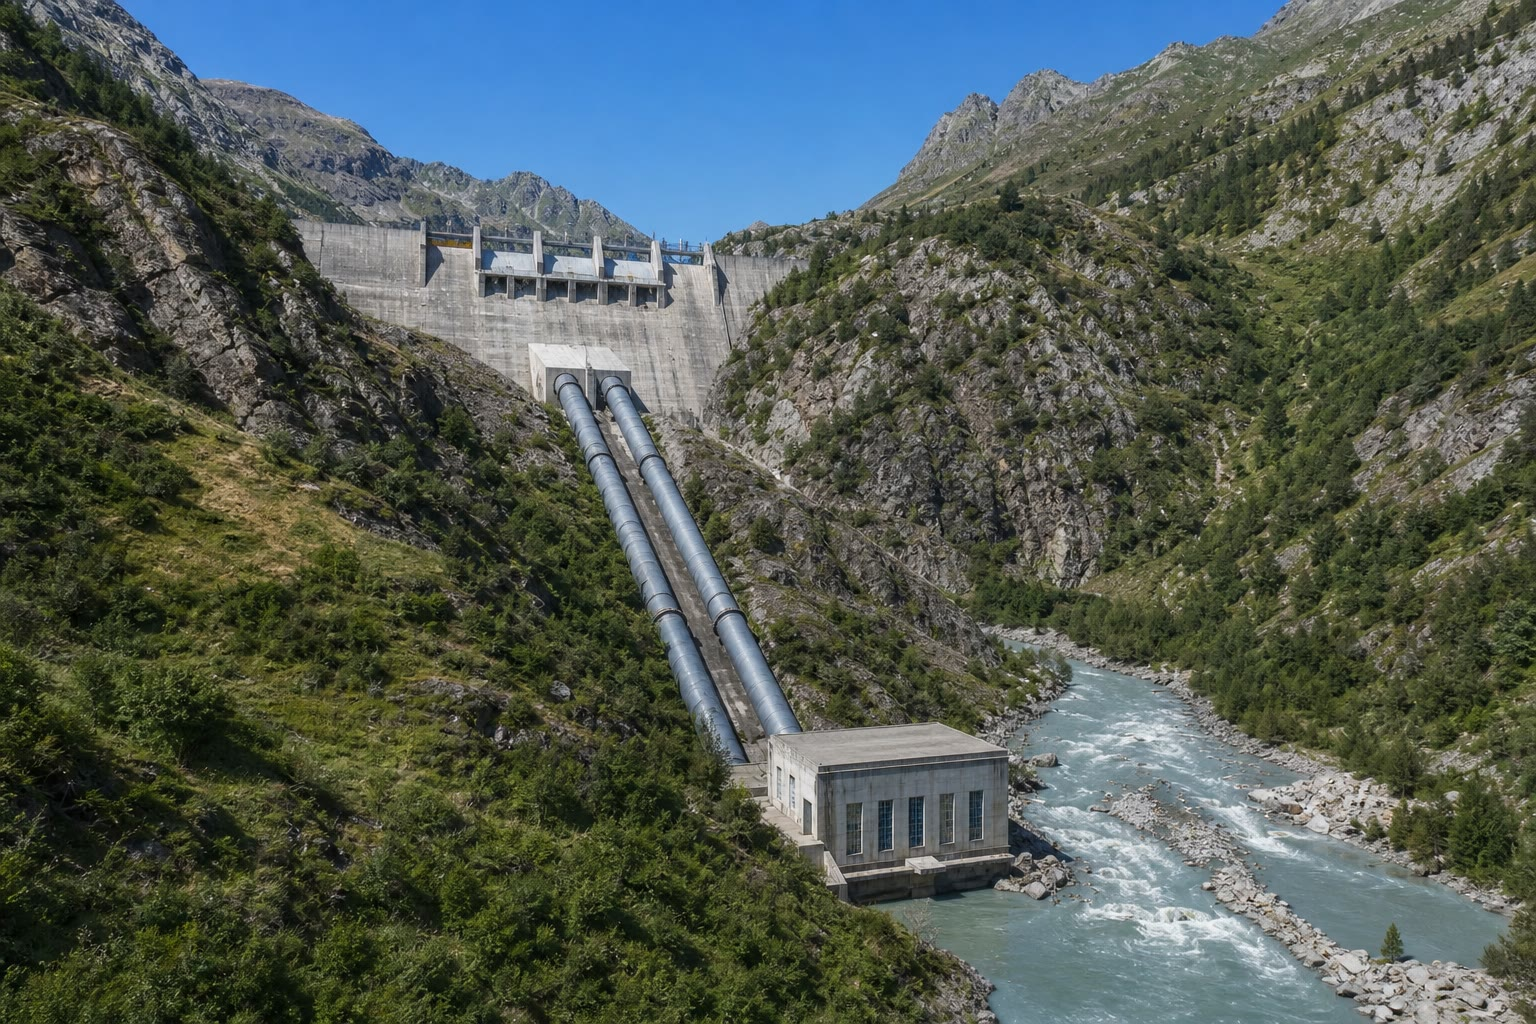
\includegraphics[width=0.58\linewidth]{images/book4/ai/b4-03-dam-penstock.jpg}

{\small Dos tuberías forzadas llevan el agua de un embalse de montaña hasta la central: doscientos metros de desnivel que el \omterm{thm:b2:euler-bernoulli:bernoulli}{teorema de Bernoulli} convierte en un chorro a sesenta metros por segundo.}
\end{omfigure}

\section{Problema: la presa, la tubería forzada y la turbina}

\begin{problem}[{Problema de fin de semana --- una central hidroeléctrica
del embalse al chorro: presiones, celeridades, potencias, pérdidas y el
golpe de ariete}]
\label{pb:b2:euler-bernoulli:1}

Un embalse retiene agua de \qty{150}{m} de profundidad tras una presa; su
superficie libre está $H = \qty{200}{m}$ por encima de las toberas de una
turbina. Una tubería forzada (de acero) de diámetro $D = \qty{3.0}{m}$ y
longitud $\ell = \qty{400}{m}$ conduce el caudal de diseño
$D_V = \qty{60}{m^3/s}$ hasta la casa de máquinas, donde una tobera lo
convierte en un chorro libre a la presión atmosférica $P_0 =
\qty{1.0}{bar}$ que golpea las cucharas de una rueda Pelton. $\rho =
\qty{1000}{kg/m^3}$, $g = \qty{9.81}{m/s^2}$; el fluido es perfecto salvo
que se diga otra cosa.

\medskip
\noindent\textbf{Parte I --- En reposo y al caudal de diseño.}
\begin{enumerate}
  \item Presión en la base de la presa y fuerza sobre una franja vertical
        de la presa, de \qty{1}{m} de ancho, de arriba abajo.
  \item Con las válvulas de la turbina cerradas, presión en la tubería
        forzada a la altura de la casa de máquinas.
  \item Celeridad en la tubería forzada al caudal de diseño; \omterm{thm:b2:euler-bernoulli:bernoulli}{presión
        dinámica} allí; presión en el extremo de la tubería junto a la casa
        de máquinas (antes de la tobera), por Bernoulli desde la
        superficie del embalse.
  \item Celeridad del chorro libre; sección y diámetro de la tobera.
  \item Potencia cinética que transporta el chorro; muéstrese que vale
        $\rho gD_VH$ y calcúlese.
  \item Masa y energía cinética del agua contenida en la tubería forzada
        al caudal de diseño; tiempo de tránsito de una partícula a lo
        largo de la tubería.
  \item Muéstrese que la carga $H$ se reparte, al caudal de diseño, entre
        la presión en el fondo de la tubería y la energía cinética del
        agua, y que la tobera convierte la primera en la segunda: ¿cuál es
        la presión justo después de la tobera?
  \item Un \omterm{def:b2:euler-bernoulli:perfect}{fluido perfecto} no tiene pérdida de carga, uno real sí: la
        pérdida en una tubería vale $\Delta P = \lambda(\ell/D)\,\tfrac12\rho v^2$ con $\lambda
        \approx 0.015$ para acero liso. Pérdida de carga en metros de agua
        y fracción de la potencia perdida.
  \item Un ingeniero propone una tubería de \qty{2}{m} para ahorrar acero.
        Repítase la pregunta 7; coméntese.
\end{enumerate}

\medskip
\noindent\textbf{Parte II --- Medir el caudal.}
Se instala un Venturi en la tubería forzada, con una garganta de \qty{2.0}{m}.
\begin{enumerate}[resume]
  \item Celeridad en la garganta y caída de presión entre la tubería y la
        garganta al caudal de diseño.
  \item La caída se lee en un manómetro de mercurio ($\rho_{\text{Hg}} =
        \qty{13600}{kg/m^3}$): diferencia de alturas.
  \item Muéstrese que el caudal es proporcional a la raíz cuadrada de la
        lectura del manómetro, y dese la lectura a la mitad del caudal de
        diseño.
  \item ¿Por qué deben las tomas de presión quedar enrasadas con la pared
        y no sobresalir hacia la corriente?
  \item Un tramo de la tubería pasa, por razones topográficas, por una
        cota \qty{6}{m} \emph{por encima} de la superficie del embalse.
        Presión allí al caudal de diseño; ¿qué ocurre y qué debe hacer el
        proyectista?
\end{enumerate}

\medskip
\noindent\textbf{Parte III --- Regímenes no estacionarios.}
El embalse tiene una superficie $A = \qty{2.0}{km^2}$.
\begin{enumerate}[resume]
  \item Velocidad a la que baja el nivel del embalse al caudal de diseño,
        en centímetros por hora.
  \item Se para la turbina y la tobera (con la sección de la pregunta 4)
        se deja abierta al aire: el embalse se vacía por gravedad.
        Escríbase el balance de masa y hállese el nivel $h(t)$ (flujo de
        Torricelli cuasiestacionario).
  \item Tiempo que tarda el nivel en bajar \qty{10}{m}; compárese con el
        tiempo al caudal de diseño constante.
  \item Puesta en marcha de la central: la tubería está llena y la tobera
        se abre en $t = 0$. Tomando la celeridad uniforme a lo largo de la
        tubería y despreciando la geometría de la tobera, intégrese Euler
        a lo largo de la conducción para obtener $\ell\,\dd v/\dd t = gH - v^2/2$,
        resuélvase y dese la constante de tiempo.
  \item Durante ese arranque, en el instante en que $v$ vale la mitad de
        su valor final, ¿cuál es la presión en el fondo de la tubería
        forzada? Explíquese el signo de la diferencia con el valor
        estacionario.
\end{enumerate}

\medskip
\noindent\textbf{Parte IV --- El cierre de la válvula.}
\begin{enumerate}[resume]
  \item La válvula de la turbina se cierra en $\tau = \qty{10}{s}$;
        supóngase que el agua de la tubería forzada se decelera
        uniformemente. Usando Euler a lo largo de la conducción, estímese
        la sobrepresión en la válvula, en bares.
  \item En un cierre rápido el agua no es incompresible: una onda de
        presión remonta la tubería a $c = \qty{1400}{m/s}$ (la celeridad
        del sonido en el agua dentro de una tubería de acero ---
        \cref{ch:b2:sound-waves}), y la sobrepresión vale
        $\Delta P = \rho c\,\Delta v$ (Joukowsky). Valor para una parada
        súbita desde el caudal de diseño; compárese con la presión
        estática. ¿Cuánto tarda la onda en llegar al embalse y volver, y
        qué dice eso sobre el significado de ``rápido''?
  \item Para proteger la tubería forzada se instala una \emph{chimenea de
        equilibrio} --- un pozo vertical abierto de sección
        $A_s = \qty{100}{m^2}$ --- allí donde un túnel horizontal de
        longitud $L = \qty{2000}{m}$ y sección $A =
        \qty{7.0}{m^2}$ procedente del embalse se une a la tubería
        forzada. Tras un cierre súbito, el agua del túnel sigue en
        movimiento y el nivel $z$ del pozo sube. Escríbase la conservación
        de la masa entre el túnel y el pozo.
  \item Intégrese Euler a lo largo del túnel (\omterm{def:b2:euler-bernoulli:perfect}{fluido perfecto}) para
        mostrar que $z$ obedece $\ddot z + \dfrac{gA}{LA_s}z = 0$; periodo
        de la oscilación.
  \item Ascenso máximo del nivel en el pozo tras un cierre desde el caudal
        de diseño (argumento energético: la energía cinética del agua del
        túnel se convierte en energía potencial en el pozo).
  \item Resúmase: las cinco presiones que aparecen en esta central
        (estática en la presa, estática en la turbina, dinámica en la
        tubería, golpe de ariete y oscilación en la chimenea) y la ley que
        da cada una.
\end{enumerate}
\end{problem}
